%% ARCHIVE 1

The \emph{photocurrent} $I_{\mathrm{Ph}}$, as shown in equation \ref{eq:photo_i}, is proportional to the radiation flux $\Phi_{\mathrm{GEN}}$ -- introduced in the previous section -- with $S = \mathrm{const.}$ being the \emph{sensitivity} of the PVC \cite{Mertens:2015}.

\begin{center}
	\begin{equation} \label{eq:photo_i}
		 I_{\mathrm{Ph}} = S \, \Phi_{\mathrm{GEN}} 
	\end{equation}
\end{center}

If now is accepted, that the diode's \emph{reverse current} $I_{\mathrm{S}}$ (diode in figure \ref{fig:tikz_solar_cell_model}) is small compared to the photocurrent $I_{\mathrm{Ph}}$, so that $I_{\mathrm{S}} + I_{\mathrm{Ph}} \approx I_{\mathrm{Ph}}$ applies, the relationship $I_{\mathrm{SC}} \approx I_{\mathrm{Ph}}$ can be derived. $I_{\mathrm{SC}}$ is the \emph{PVG short circuit current}.

Based on this, the PVG's short circuit current $I_{\mathrm{SC, \vartheta}}$ depending on the \emph{PVC temperature} $\vartheta_{\mathrm{PVC}}$, taking into account the \emph{temperature coefficient} of the short circuit current\footnote{Typical $\mathrm{TC}\left(I_{\mathrm{SC}}\right)$ values for Si-PVCs are around $0,06 \% / \mathrm{K}$.} $\mathrm{TC}\left(I_{\mathrm{SC}}\right)$, can be approximated to:
\begin{center}
	\begin{equation} \label{eq:i_short_circuit}
		I_{\mathrm{SC, \vartheta}} \approx I_{\mathrm{Ph}} \, \left[ 1 + \mathrm{TC}\left(I_{\mathrm{SC}}\right) \cdot \left(\vartheta_{\mathrm{PVC}} - \vartheta_{\mathrm{STC}} \right) \right] \text{.}
	\end{equation}
\end{center}
The temperature coefficient $\mathrm{TC}\left(I_{\mathrm{SC}}\right)$ can usually be obtained from a PVG's data sheet. And the temperature of the PVCs at \emph{standard test conditions} (STC) $\vartheta_{\mathrm{STC}}$ can be taken from table \ref{tab:table_STC}. These are the conditions under which the paramaters in the data sheet of a PVG apply \cite{Mertens:2015, Wagner:2018}. 

\begin{table}[h!]
	\centering
	\footnotesize
\begin{tabular}{|l|c|}
	\hline
	\multicolumn{2}{|c|}{\textbf{Standard test conditions for PV generators}} \\
	\hline
 	Total irradiance received by the PV generator & $E_{\mathrm{STC}} = 1000\mathrm{W} \mathrm{m}^{-2}$ \\
	PV cell temperature & $\vartheta_{\mathrm{STC}} = 25^\circ \mathrm{C}$ \\
	Solar spectrum & AM 1,5 \\
	\hline
\end{tabular}
	\caption{Parameters for the standard test conditions of a photovoltaic generator \cite{Mertens:2015}.}
	\label{tab:table_STC}
\end{table}

Furthermore, the PVC temperature $\vartheta_{\mathrm{PVC}}$, depending on the total irradiance $E_{\mathrm{GEN}}$ and the \emph{ambient temperature} $\vartheta_{\mathrm{A}}$, with the \emph{nominal operating cell temperature}\footnote{Typical $\mathrm{NOCT}$ values for c-Si-PVGs are around $45$ to $50^\circ \mathrm{C}$.} $\mathrm{NOCT}$ and the conditions under which it is measured, $\vartheta_{\mathrm{A,NOCT}}$ and $E_{\mathrm{NOCT}}$, can be approximated by assuming that the increase of $\vartheta_{\mathrm{PVC}}$ compared to the ambient temperature $\vartheta_{\mathrm{A}}$ is proportional to $E_{\mathrm{GEN}}$:
\begin{center}
	\begin{equation} \label{eq:cell_temp}
		\vartheta_{\mathrm{PVC}} \approx \vartheta_{\mathrm{A}} + \left(\mathrm{NOCT} - \vartheta_{\mathrm{A,NOCT}}\right) \frac{E_{\mathrm{GEN}}}{E_{\mathrm{NOCT}}} \text{.}
	\end{equation}
\end{center}
The paramateres under which the $\mathrm{NOCT}$ is measured are provided by table \ref{tab:table_NOCT} and -- in addition to $\mathrm{TC}\left(I_{\mathrm{SC}}\right)$ -- the $\mathrm{NOCT}$ is usually listed in the PVG's data sheet \cite{Mertens:2015}.

\begin{table}[h!]
	\centering
	\footnotesize
\begin{tabular}{|l|c|}
	\hline
	\multicolumn{2}{|c|}{\textbf{Conditions for NOCT measurement}} \\
	\hline
 	Total irradiance received by the PV generator & $E_{\mathrm{NOCT}} = 800\mathrm{W} \mathrm{m}^{-2}$ \\
	Ambient temperature & $\vartheta_{\mathrm{A, NOCT}} = 20^\circ \mathrm{C}$ \\
	Wind speed & $v_{\mathrm W} = 1 \mathrm{m} \mathrm{s}^{-1}$  \\
	\hline
\end{tabular}
	\caption{Conditions under which the NOCT is measured \cite{Mertens:2015}.}
	\label{tab:table_NOCT}
\end{table}

Ambient temperatures $\vartheta_{\mathrm{A}}$ for different locations on Earth can be obtained from climate charts. Figure \ref{fig:temp_vienna} provides data for monthly averages of temperature in $^\circ \mathrm{C}$ and precipitation in $\mathrm{mm}$, collected by the Global Historical Climatology Network, for the Hohe Warte in Vienna, Austria, between 1997 and 2016. Below the chart the percentage of missing data regarding the months of the year, is presented. More climate charts can be found in appendix \ref{ap:solar_resource_maps} \cite{Zepner:2020}.

\begin{figure}[h!]
	\centering
  	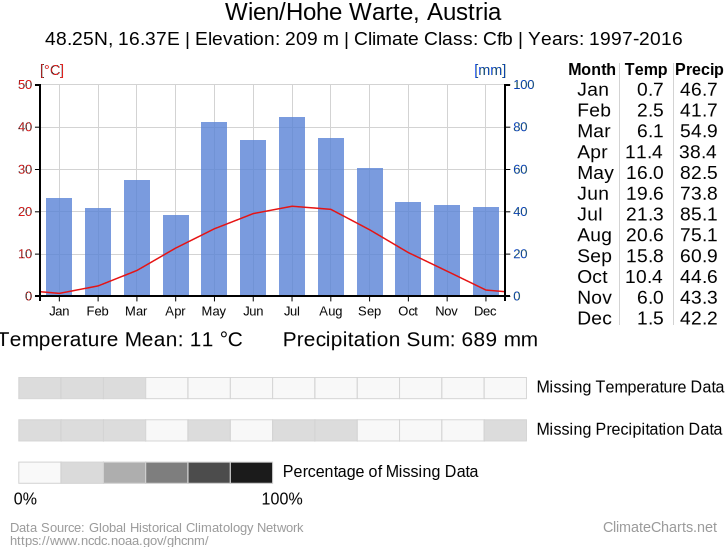
\includegraphics[width = 0.96\textwidth]{temp_maps/temp_vienna}
  	\caption{Monthly averages of temperature and precipitation data for the Hohe Warte in Vienna, Austria. (Image credit: \cite{Zepner:2020} and \emph{climatecharts.net})}
	\label{fig:temp_vienna}
\end{figure}

After applying Kirchoff's first law to the simplified PVC model in figure \ref{fig:tikz_solar_cell_model} and taking equations \ref{eq:u_pvg_sum_of_pvc} and \ref{eq:i_short_circuit} into account, the PVG's effective current-voltage characteristic, depending on the radiation flux $\Phi_{\mathrm{GEN}}$ and the PVC temperature $\vartheta_{\mathrm{PVC}}$, can be modeled with the following equations:
\begin{center}
	\begin{equation} \label{eq:i_of_u}
		I_{\mathrm{PVG}}\left(U_{\mathrm{PVG}}\right) = I_{\mathrm{SC},\vartheta} - \underbrace{I_{\mathrm{S}} \left( \exp \left( \frac{1}{U_{\mathrm{T}}} \left( \frac{U_{\mathrm{PVG}}}{N_{\mathrm{PVC}}} + I_{\mathrm{PVG}} \, R_{\mathrm{PV}} \right) \right) - 1  \right)}_{I_{\mathrm{D}}} \text{,}
	\end{equation}
\end{center}
\begin{center}
	\begin{equation} \label{eq:u_of_i}
		U_{\mathrm{PVG}}\left(I_{\mathrm{PVG}}\right) = N_{\mathrm{PVC}} \left( U_{\mathrm{T}} \, \ln \left( \frac{I_{\mathrm{SC}, \vartheta} - I_{\mathrm{PVG}} + I_{\mathrm{S}}}{I_{\mathrm{S}}} \right) - I_{\mathrm{PVG}} \, R_{\mathrm{PV}} \right) \text{.}
	\end{equation}
\end{center}
$U_{\mathrm{T}}$ is the diodes's \emph{thermal voltage} and it can be obtained from equation \ref{eq:u_temp}, with $k = 1,380649 \cdot 10^{-23} \mathrm{Ws/K}$ being the Bolzmann constant and $e = 1,602176634\cdot10^{-19} \mathrm{As}$ being the elementary charge.
\begin{center}
	\begin{equation} \label{eq:u_temp}
		U_{\mathrm{T}} = \frac{ k \, \left( \vartheta_{\mathrm{PVC}} + 273,15^\circ \mathrm{C} \right) }{e} \cdot \frac{\mathrm{K}}{^\circ \mathrm{C}}
	\end{equation}
\end{center}
The corresponding curve of the PVG current $I_{\mathrm{PVG}}$ as a function of the PVG voltage $U_{\mathrm{PVG}}$, is shown in figure \ref{fig:tikz/tikz_PVG_curve}. MPP is the \emph{maximum power point} for which the greatest electrical power, $P_{\mathrm{MPP}} = U_{\mathrm{MPP}} \, I_{\mathrm{MPP}}$, is provided by the PVG.
\begin{figure}[h!]
	\centering
	

\tikzset{every picture/.style={line width=0.75pt}} %set default line width to 0.75pt        

\begin{tikzpicture}[x=0.75pt,y=0.75pt,yscale=-1,xscale=1]
%uncomment if require: \path (0,300); %set diagram left start at 0, and has height of 300

%Image [id:dp8816301757772553] 
\draw (309.25,160) node [xscale=-1] {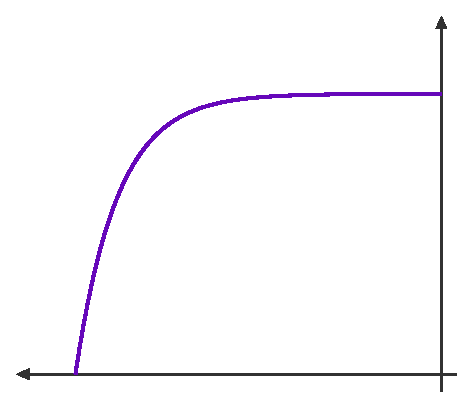
\includegraphics[width=211.13pt,height=180pt]{images/image_PVC_curve}};
%Straight Lines [id:da8531224351110531] 
\draw [color={rgb, 255:red, 155; green, 155; blue, 155 }  ,draw opacity=1 ] [dash pattern={on 4.5pt off 4.5pt}]  (184,113) -- (358,113) ;
%Straight Lines [id:da1728021335997585] 
\draw [color={rgb, 255:red, 155; green, 155; blue, 155 }  ,draw opacity=1 ] [dash pattern={on 4.5pt off 4.5pt}]  (358,113) -- (358,269) ;
%Shape: Circle [id:dp9850794530438081] 
\draw  [fill={rgb, 255:red, 255; green, 255; blue, 255 }  ,fill opacity=1 ] (356,113) .. controls (356,111.9) and (356.9,111) .. (358,111) .. controls (359.1,111) and (360,111.9) .. (360,113) .. controls (360,114.1) and (359.1,115) .. (358,115) .. controls (356.9,115) and (356,114.1) .. (356,113) -- cycle ;

% Text Node
\draw (129,19.4) node [anchor=north west][inner sep=0.75pt]  [font=\footnotesize]  {$I_{\mathrm{PV}}( U_{\mathrm{PV}} ,\vartheta _{\mathrm{C}} ,\Phi _{\mathrm{G}})$};
% Text Node
\draw (456,263.4) node [anchor=north west][inner sep=0.75pt]  [font=\footnotesize]  {$U_{\mathrm{PV}}$};
% Text Node
\draw (278,276.4) node [anchor=north west][inner sep=0.75pt]  [font=\footnotesize]  {$U_{\mathrm{MPP}}( \vartheta _{\mathrm{C}} ,\Phi _{\mathrm{G}})$};
% Text Node
\draw (91,105.4) node [anchor=north west][inner sep=0.75pt]  [font=\footnotesize]  {$I_{\mathrm{MPP}}( \vartheta _{\mathrm{C}} ,\Phi _{\mathrm{G}})$};
% Text Node
\draw (361,96) node [anchor=north west][inner sep=0.75pt]  [font=\footnotesize] [align=left] {MPP};
% Text Node
\draw (370,276.4) node [anchor=north west][inner sep=0.75pt]  [font=\footnotesize]  {$U_{\mathrm{OC}}( \vartheta _{\mathrm{C}} ,\Phi _{\mathrm{G}})$};
% Text Node
\draw (102,83.4) node [anchor=north west][inner sep=0.75pt]  [font=\footnotesize]  {$I_{\mathrm{SC}}( \vartheta _{\mathrm{C}} ,\Phi _{\mathrm{G}})$};
% Text Node
\draw (166,273.4) node [anchor=north west][inner sep=0.75pt]  [font=\footnotesize]  {$0$};


\end{tikzpicture}


	\caption{Modeled current-voltage characteristic of a photovoltaic generator depending on the radiation flux $\Phi_{\mathrm{GEN}}$ and the photovoltaic cell temperature $\vartheta_{\mathrm{PVC}}$.}
	\label{fig:tikz/tikz_PVG_curve}
\end{figure}
With the effective current-voltage characteristic, the engineering of the characteristic of the PVG to solve adaptation problem, with an accuracy of 1\% related to $P_{\mathrm{MPP}}$, is possible \cite{Prechtl:2006, Mertens:2015, Tietze:2016, Wagner:2018, Elert:2020}.

Upon closer inspection of equation \ref{eq:i_of_u} for $I_{\mathrm{PVG}} = 0\mathrm{A}$, while taking equation \ref{eq:u_pvg_sum_of_pvc} into account, the diode's reverse current $I_{\mathrm{S}}$ can be derived to:\footnote{As for equation \ref{eq:i_short_circuit}, $I_{\mathrm{S}} + I_{\mathrm{Ph}} \approx I_{\mathrm{Ph}}$, is assumed.}
\begin{center}
	\begin{equation} \label{eq:reverse_current}
		I_{\mathrm{S}} \approx I_{\mathrm{SC, \vartheta}} \, \exp \left(-\frac{U_{\mathrm{OC, \vartheta}}}{U_{\mathrm{T}} \, N_{\mathrm{PVC}}}\right) \text{.}
	\end{equation}
\end{center}
And since $I_{\mathrm{S}}$ depends on the physical structure of the PVC, it can be calcultated with $I_{\mathrm{SC,STC}}$ and $U_{\mathrm{OC,STC}}$ from a PVG's data sheet. Once its value is determined, the temperature dependent \emph{open circuit voltage} $U_{\mathrm{OC,\vartheta}}$ of a PVG can be calculated by transforming this equation \cite{Mertens:2015, Wagner:2018}.\footnote{Equation \ref{eq:reverse_current} can be derived from equation \ref{eq:u_of_i} for $I_{\mathrm{PVG}} = 0\mathrm{A}$.}

It was mentioned earlier, that the simplified model from figure \ref{fig:tikz_solar_cell_model} has a very good approximation quality. This statement is only valid if the \emph{series resistance} $R_{\mathrm{PV}}$ of the PVC is allowed to take on negative values. And since resistors cannot have negative values, it is a fictitious photoelectric component with the aim of approximating the actual current-voltage characteristic of a PVG. Therefore it does not necessarily have to have a physical meaning \cite{Wagner:2018}.

\begin{center}
	\begin{equation} \label{eq:d_U_to_d_I}
		M = \frac{\mathrm{d} U_{\mathrm{PVG}}}{\mathrm{d} I_{\mathrm{PVG}}}\left(I_{\mathrm{PVG}} = 0\mathrm{A}\right) = - N_{\mathrm{PVC}} \left( \frac{U_{\mathrm{T}}}{I_{\mathrm{SC, \vartheta}} + I_{\mathrm{S}}} + R_{\mathrm{PV}} \right)
	\end{equation}
\end{center}

\begin{center}
	\begin{equation} \label{eq:r_pv_with_M}
		R_{\mathrm{PV}} = - M \, \frac{I_{\mathrm{SC, \vartheta}}}{I_{\mathrm{MPP}}} + \frac{U_{\mathrm{MPP}}}{I_{\mathrm{MPP}}} \left(1 - \frac{I_{\mathrm{SC, \vartheta}}}{I_{\mathrm{MPP}}} \right) 
	\end{equation}
\end{center}

\begin{center}
	\begin{equation} \label{eq:r_pv}
		R_{\mathrm{PV}} = \left[ N_{\mathrm{PVC}} \, U_{\mathrm{T}} \, \frac{I_{\mathrm{SC, \vartheta}}}{I_{\mathrm{SC, \vartheta}} + I_{\mathrm{S}}} + U_{\mathrm{MPP}} \, \left(1 - \frac{I_{\mathrm{SC, \vartheta}}}{I_{\mathrm{MPP}}} \right) \right] \left( I_{\mathrm{MPP}} - N_{\mathrm{PVC}} \, I_{\mathrm{SC, \vartheta}}\right)^{-1}
	\end{equation}
\end{center}

%% END ARCHIVE 1







%% ARCHIVE 2

In the next step, the PVCs shown in figure \ref{fig:tikz_PVG_circuit_diagram}, must be modeled. For this, the simplified PVC model\footnote{This model is derived from the PVC standard model for $R_{\mathrm{P}} \to \infty$ \cite{Mertens:2015, Wagner:2018}.} is used, as there is an explicit solution for $U_{\mathrm{PVC}}$, while at the same time an approximation quality similar to the two-diode model can be achieved. This statement however, is only valid if the \emph{series resistance} $R_{\mathrm{PV}}$ of the PVC is allowed to take on negative values. And because resistors cannot have negative values, it is treated as a fictitious photoelectric component that is used to approximate the actual current-voltage characteristic of a PVG. An illustration of the simplified PVC model with $R_{\mathrm{PV}}$ is provided in figure \ref{fig:tikz_PVC_simplified} \cite{Wagner:2018}.

\begin{figure}[h!]
	\centering
	

\tikzset{every picture/.style={line width=0.75pt}} %set default line width to 0.75pt        

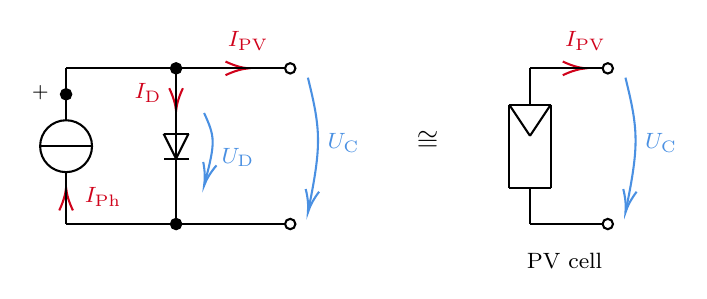
\begin{tikzpicture}[x=0.75pt,y=0.75pt,yscale=-1,xscale=1]
%uncomment if require: \path (0,391); %set diagram left start at 0, and has height of 391

%Straight Lines [id:da9220046892300695] 
\draw [color={rgb, 255:red, 208; green, 2; blue, 27 }  ,draw opacity=1 ]   (259.5,142.5) -- (273.25,142.5) ;
\draw [shift={(275.25,142.5)}, rotate = 180] [color={rgb, 255:red, 208; green, 2; blue, 27 }  ,draw opacity=1 ][line width=0.75]    (10.93,-3.29) .. controls (6.95,-1.4) and (3.31,-0.3) .. (0,0) .. controls (3.31,0.3) and (6.95,1.4) .. (10.93,3.29)   ;
%Straight Lines [id:da9695421868123493] 
\draw [color={rgb, 255:red, 208; green, 2; blue, 27 }  ,draw opacity=1 ]   (422,142.5) -- (435.75,142.5) ;
\draw [shift={(437.75,142.5)}, rotate = 180] [color={rgb, 255:red, 208; green, 2; blue, 27 }  ,draw opacity=1 ][line width=0.75]    (10.93,-3.29) .. controls (6.95,-1.4) and (3.31,-0.3) .. (0,0) .. controls (3.31,0.3) and (6.95,1.4) .. (10.93,3.29)   ;
%Straight Lines [id:da29339333794333666] 
\draw [color={rgb, 255:red, 208; green, 2; blue, 27 }  ,draw opacity=1 ]   (240.5,142.5) -- (240.5,161) ;
\draw [shift={(240.5,163)}, rotate = 270] [color={rgb, 255:red, 208; green, 2; blue, 27 }  ,draw opacity=1 ][line width=0.75]    (10.93,-3.29) .. controls (6.95,-1.4) and (3.31,-0.3) .. (0,0) .. controls (3.31,0.3) and (6.95,1.4) .. (10.93,3.29)   ;
%Straight Lines [id:da5182268392298646] 
\draw [color={rgb, 255:red, 208; green, 2; blue, 27 }  ,draw opacity=1 ]   (187.5,212.5) -- (187.5,202) ;
\draw [shift={(187.5,200)}, rotate = 450] [color={rgb, 255:red, 208; green, 2; blue, 27 }  ,draw opacity=1 ][line width=0.75]    (10.93,-3.29) .. controls (6.95,-1.4) and (3.31,-0.3) .. (0,0) .. controls (3.31,0.3) and (6.95,1.4) .. (10.93,3.29)   ;
%Straight Lines [id:da19579076658988703] 
\draw    (187.5,192.5) -- (187.5,217.5) ;
%Straight Lines [id:da500967170364542] 
\draw    (240.5,142.5) -- (240.5,217.5) ;
%Straight Lines [id:da9693092867247253] 
\draw    (187.5,142.5) -- (187.5,167.5) ;
%Straight Lines [id:da3180920793144646] 
\draw    (240.5,186) -- (234.5,186) ;
%Straight Lines [id:da3231236229149821] 
\draw    (246.5,186) -- (240.5,186) ;
%Straight Lines [id:da20274569848223778] 
\draw    (246.5,174) -- (240.5,174) ;
%Straight Lines [id:da4237476648515044] 
\draw    (240.5,174) -- (234.5,174) ;
%Straight Lines [id:da7091520922682297] 
\draw    (234.5,174) -- (240.5,186) ;
%Straight Lines [id:da8216387087718504] 
\draw    (240.5,186) -- (246.5,174) ;
%Shape: Circle [id:dp46632786849059626] 
\draw   (175,180) .. controls (175,173.1) and (180.6,167.5) .. (187.5,167.5) .. controls (194.4,167.5) and (200,173.1) .. (200,180) .. controls (200,186.9) and (194.4,192.5) .. (187.5,192.5) .. controls (180.6,192.5) and (175,186.9) .. (175,180) -- cycle ;
%Straight Lines [id:da6428722008154575] 
\draw    (175,180) -- (200,180) ;
%Shape: Circle [id:dp9143776877359857] 
\draw  [fill={rgb, 255:red, 0; green, 0; blue, 0 }  ,fill opacity=1 ] (238,217.5) .. controls (238,216.12) and (239.12,215) .. (240.5,215) .. controls (241.88,215) and (243,216.12) .. (243,217.5) .. controls (243,218.88) and (241.88,220) .. (240.5,220) .. controls (239.12,220) and (238,218.88) .. (238,217.5) -- cycle ;
%Shape: Circle [id:dp04116434903611532] 
\draw  [fill={rgb, 255:red, 0; green, 0; blue, 0 }  ,fill opacity=1 ] (185,155) .. controls (185,153.62) and (186.12,152.5) .. (187.5,152.5) .. controls (188.88,152.5) and (190,153.62) .. (190,155) .. controls (190,156.38) and (188.88,157.5) .. (187.5,157.5) .. controls (186.12,157.5) and (185,156.38) .. (185,155) -- cycle ;
%Shape: Circle [id:dp7561083964816784] 
\draw  [fill={rgb, 255:red, 0; green, 0; blue, 0 }  ,fill opacity=1 ] (238,142.5) .. controls (238,141.12) and (239.12,140) .. (240.5,140) .. controls (241.88,140) and (243,141.12) .. (243,142.5) .. controls (243,143.88) and (241.88,145) .. (240.5,145) .. controls (239.12,145) and (238,143.88) .. (238,142.5) -- cycle ;
%Curve Lines [id:da12939293693438314] 
\draw [color={rgb, 255:red, 74; green, 144; blue, 226 }  ,draw opacity=1 ]   (254,164) .. controls (259.33,175.64) and (259.5,177.87) .. (254.48,197.16) ;
\draw [shift={(254,199)}, rotate = 284.68] [color={rgb, 255:red, 74; green, 144; blue, 226 }  ,draw opacity=1 ][line width=0.75]    (10.93,-3.29) .. controls (6.95,-1.4) and (3.31,-0.3) .. (0,0) .. controls (3.31,0.3) and (6.95,1.4) .. (10.93,3.29)   ;
%Straight Lines [id:da820440930056753] 
\draw    (401,160) -- (421,160) ;
%Straight Lines [id:da5978422659023195] 
\draw    (401,160) -- (411,175) ;
%Straight Lines [id:da8646077617642114] 
\draw    (411,175) -- (421,160) ;
%Straight Lines [id:da1683854382748906] 
\draw    (401,160) -- (401,200) ;
%Straight Lines [id:da35944219412656886] 
\draw    (421,160) -- (421,200) ;
%Straight Lines [id:da012841517263090685] 
\draw    (401,200) -- (421,200) ;
%Straight Lines [id:da8937999883743217] 
\draw    (411,200) -- (411,217.5) ;
%Shape: Circle [id:dp39581519495881] 
\draw   (446,142.5) .. controls (446,141.12) and (447.12,140) .. (448.5,140) .. controls (449.88,140) and (451,141.12) .. (451,142.5) .. controls (451,143.88) and (449.88,145) .. (448.5,145) .. controls (447.12,145) and (446,143.88) .. (446,142.5) -- cycle ;
%Shape: Circle [id:dp7404102366707606] 
\draw   (446,217.5) .. controls (446,216.12) and (447.12,215) .. (448.5,215) .. controls (449.88,215) and (451,216.12) .. (451,217.5) .. controls (451,218.88) and (449.88,220) .. (448.5,220) .. controls (447.12,220) and (446,218.88) .. (446,217.5) -- cycle ;
%Straight Lines [id:da16056380159184358] 
\draw    (411,142.5) -- (446,142.5) ;
%Straight Lines [id:da8365114488683654] 
\draw    (411,217.5) -- (446,217.5) ;
%Curve Lines [id:da5511080558248806] 
\draw [color={rgb, 255:red, 74; green, 144; blue, 226 }  ,draw opacity=1 ]   (457,147) .. controls (463.37,172.48) and (463.5,179.71) .. (457.38,210.11) ;
\draw [shift={(457,212)}, rotate = 281.48] [color={rgb, 255:red, 74; green, 144; blue, 226 }  ,draw opacity=1 ][line width=0.75]    (10.93,-3.29) .. controls (6.95,-1.4) and (3.31,-0.3) .. (0,0) .. controls (3.31,0.3) and (6.95,1.4) .. (10.93,3.29)   ;
%Straight Lines [id:da725857721119765] 
\draw    (411,142.5) -- (411,160) ;
%Straight Lines [id:da5740090703572132] 
\draw    (187.5,142.5) -- (240.5,142.5) ;
%Straight Lines [id:da4778393661136311] 
\draw    (187.5,217.5) -- (240.5,217.5) ;
%Shape: Circle [id:dp2917985814178987] 
\draw   (293,142.5) .. controls (293,141.12) and (294.12,140) .. (295.5,140) .. controls (296.88,140) and (298,141.12) .. (298,142.5) .. controls (298,143.88) and (296.88,145) .. (295.5,145) .. controls (294.12,145) and (293,143.88) .. (293,142.5) -- cycle ;
%Shape: Circle [id:dp07126668235633615] 
\draw   (293,217.5) .. controls (293,216.12) and (294.12,215) .. (295.5,215) .. controls (296.88,215) and (298,216.12) .. (298,217.5) .. controls (298,218.88) and (296.88,220) .. (295.5,220) .. controls (294.12,220) and (293,218.88) .. (293,217.5) -- cycle ;
%Curve Lines [id:da8740596681425179] 
\draw [color={rgb, 255:red, 74; green, 144; blue, 226 }  ,draw opacity=1 ]   (304,147) .. controls (310.37,172.48) and (310.5,179.71) .. (304.38,210.11) ;
\draw [shift={(304,212)}, rotate = 281.48] [color={rgb, 255:red, 74; green, 144; blue, 226 }  ,draw opacity=1 ][line width=0.75]    (10.93,-3.29) .. controls (6.95,-1.4) and (3.31,-0.3) .. (0,0) .. controls (3.31,0.3) and (6.95,1.4) .. (10.93,3.29)   ;
%Straight Lines [id:da2745454915751546] 
\draw    (240.5,142.5) -- (293.5,142.5) ;
%Straight Lines [id:da3914094245668047] 
\draw    (240.5,217.5) -- (293.5,217.5) ;

% Text Node
\draw (219,148.4) node [anchor=north west][inner sep=0.75pt]  [font=\footnotesize,color={rgb, 255:red, 208; green, 2; blue, 27 }  ,opacity=1 ]  {$I_{\mathrm{D}}$};
% Text Node
\draw (195,198.4) node [anchor=north west][inner sep=0.75pt]  [font=\footnotesize,color={rgb, 255:red, 208; green, 2; blue, 27 }  ,opacity=1 ]  {$I_{\mathrm{Ph}}$};
% Text Node
\draw (261,179.4) node [anchor=north west][inner sep=0.75pt]  [font=\footnotesize,color={rgb, 255:red, 74; green, 144; blue, 226 }  ,opacity=1 ]  {$U_{\mathrm{D}}$};
% Text Node
\draw (355,171.4) node [anchor=north west][inner sep=0.75pt]  [font=\normalsize]  {$\cong $};
% Text Node
\draw (465,172.4) node [anchor=north west][inner sep=0.75pt]  [font=\footnotesize,color={rgb, 255:red, 74; green, 144; blue, 226 }  ,opacity=1 ]  {$U_{\mathrm{C}}$};
% Text Node
\draw (426.5,123.4) node [anchor=north west][inner sep=0.75pt]  [font=\footnotesize,color={rgb, 255:red, 208; green, 2; blue, 27 }  ,opacity=1 ]  {$I_{\mathrm{PV}}$};
% Text Node
\draw (408,230) node [anchor=north west][inner sep=0.75pt]  [font=\footnotesize] [align=left] {PV cell};
% Text Node
\draw (312,172.4) node [anchor=north west][inner sep=0.75pt]  [font=\footnotesize,color={rgb, 255:red, 74; green, 144; blue, 226 }  ,opacity=1 ]  {$U_{\mathrm{C}}$};
% Text Node
\draw (264,123.4) node [anchor=north west][inner sep=0.75pt]  [font=\footnotesize,color={rgb, 255:red, 208; green, 2; blue, 27 }  ,opacity=1 ]  {$I_{\mathrm{PV}}$};
% Text Node
\draw (169.5,149.4) node [anchor=north west][inner sep=0.75pt]  [font=\scriptsize]  {$+$};


\end{tikzpicture}

	\caption{Simplified standard model of a photovoltaic cell. (Image credit: \cite{Mertens:2015, Wagner:2018})}
	\label{fig:tikz_PVC_simplified}
\end{figure}

After applying Kirchoff's first law to the simplified PVC model and taking equation \ref{eq:u_pvg_sum_of_pvc} into account, the PVG's effective current-voltage characteristic can be modeled with the equation \ref{eq:i_of_u}, in which $I_{\mathrm{S}}$ is the diode's \emph{reverse current}, $U_{\mathrm{T}}$ its \emph{thermal voltage} and $I_{\mathrm{Ph}} = I_{\mathrm{Ph}}\left(\Phi\right)$, depending on the radiation flux $\Phi = \Phi_{\mathrm{GEN}}$, is the PVC's \emph{photocurrent}.
\begin{center}
	\begin{equation} \label{eq:i_of_u}
		I_{\mathrm{PVG}}\left(U_{\mathrm{PVG}}\right) = I_{\mathrm{Ph}} - \underbrace{I_{\mathrm{S}} \left( \exp \left( \frac{1}{U_{\mathrm{T}}} \left( \frac{U_{\mathrm{PVG}}}{N_{\mathrm{PVC}}} + I_{\mathrm{PVG}} \, R_{\mathrm{PV}} \right) \right) - 1  \right)}_{I_{\mathrm{D}}}
	\end{equation}
\end{center}
The explicit solution for $U_{\mathrm{PVC}}$, as shown in equation \ref{eq:u_of_i}, can be derived by transforming equation \ref{eq:i_of_u} \cite{Mertens:2015, Tietze:2016, Wagner:2018}. 
\begin{center}
	\begin{equation} \label{eq:u_of_i}
		U_{\mathrm{PVG}}\left(I_{\mathrm{PVG}}\right) = N_{\mathrm{PVC}} \left( U_{\mathrm{T}} \, \ln \left( \frac{I_{\mathrm{Ph}} - I_{\mathrm{PVG}} + I_{\mathrm{S}}}{I_{\mathrm{S}}} \right) - I_{\mathrm{PVG}} \, R_{\mathrm{PV}} \right)
	\end{equation}
\end{center}

Based on equation \ref{eq:i_of_u} the effective current-voltage characteristic can be visualized as shown in figure \ref{fig:tikz/tikz_PVG_curve}. $I_{\mathrm{SC}}\left(\vartheta,\Phi\right)$ and $U_{\mathrm{OC}}\left(\vartheta,\Phi\right)$ are the PVG's \emph{short-circuit} current and \emph{open-circuit} voltage, which depend on the PVC temperature $\vartheta = \vartheta_{\mathrm{PVC}}$ and the radiation flux $\Phi = \Phi_{\mathrm{GEN}}$, and the MPP is the \emph{maximum power point}, for which the PVG provides the greatest electrical power:
\begin{center}
	\begin{equation} \label{eq:p_mpp}
		P_{\mathrm{MPP}} = U_{\mathrm{MPP}} \, I_{\mathrm{MPP}} \text{.}
	\end{equation}
\end{center}
With the effective current-voltage characteristic, the actual current-voltage characteristic of the PVG can be modeled with an accuracy of 1\% related to $P_{\mathrm{MPP}}$ \cite{Prechtl:2006, Mertens:2015, Wagner:2018}.\footnote{A greater accuracy can be achieved by using the Newton-Raphson iteration method to determine the unknown quantities in the following paragraph \cite{Wagner:2018}.}
\begin{figure}[h!]
	\centering
	

\tikzset{every picture/.style={line width=0.75pt}} %set default line width to 0.75pt        

\begin{tikzpicture}[x=0.75pt,y=0.75pt,yscale=-1,xscale=1]
%uncomment if require: \path (0,300); %set diagram left start at 0, and has height of 300

%Image [id:dp8816301757772553] 
\draw (309.25,160) node [xscale=-1] {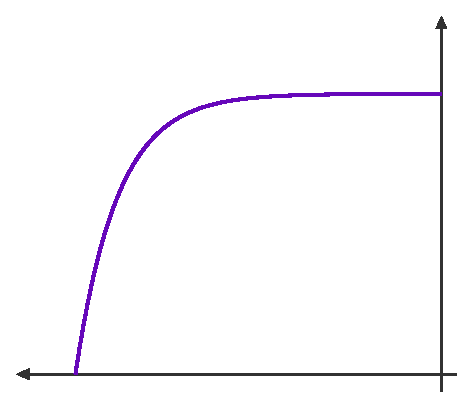
\includegraphics[width=211.13pt,height=180pt]{images/image_PVC_curve}};
%Straight Lines [id:da8531224351110531] 
\draw [color={rgb, 255:red, 155; green, 155; blue, 155 }  ,draw opacity=1 ] [dash pattern={on 4.5pt off 4.5pt}]  (184,113) -- (358,113) ;
%Straight Lines [id:da1728021335997585] 
\draw [color={rgb, 255:red, 155; green, 155; blue, 155 }  ,draw opacity=1 ] [dash pattern={on 4.5pt off 4.5pt}]  (358,113) -- (358,269) ;
%Shape: Circle [id:dp9850794530438081] 
\draw  [fill={rgb, 255:red, 255; green, 255; blue, 255 }  ,fill opacity=1 ] (356,113) .. controls (356,111.9) and (356.9,111) .. (358,111) .. controls (359.1,111) and (360,111.9) .. (360,113) .. controls (360,114.1) and (359.1,115) .. (358,115) .. controls (356.9,115) and (356,114.1) .. (356,113) -- cycle ;

% Text Node
\draw (129,19.4) node [anchor=north west][inner sep=0.75pt]  [font=\footnotesize]  {$I_{\mathrm{PV}}( U_{\mathrm{PV}} ,\vartheta _{\mathrm{C}} ,\Phi _{\mathrm{G}})$};
% Text Node
\draw (456,263.4) node [anchor=north west][inner sep=0.75pt]  [font=\footnotesize]  {$U_{\mathrm{PV}}$};
% Text Node
\draw (278,276.4) node [anchor=north west][inner sep=0.75pt]  [font=\footnotesize]  {$U_{\mathrm{MPP}}( \vartheta _{\mathrm{C}} ,\Phi _{\mathrm{G}})$};
% Text Node
\draw (91,105.4) node [anchor=north west][inner sep=0.75pt]  [font=\footnotesize]  {$I_{\mathrm{MPP}}( \vartheta _{\mathrm{C}} ,\Phi _{\mathrm{G}})$};
% Text Node
\draw (361,96) node [anchor=north west][inner sep=0.75pt]  [font=\footnotesize] [align=left] {MPP};
% Text Node
\draw (370,276.4) node [anchor=north west][inner sep=0.75pt]  [font=\footnotesize]  {$U_{\mathrm{OC}}( \vartheta _{\mathrm{C}} ,\Phi _{\mathrm{G}})$};
% Text Node
\draw (102,83.4) node [anchor=north west][inner sep=0.75pt]  [font=\footnotesize]  {$I_{\mathrm{SC}}( \vartheta _{\mathrm{C}} ,\Phi _{\mathrm{G}})$};
% Text Node
\draw (166,273.4) node [anchor=north west][inner sep=0.75pt]  [font=\footnotesize]  {$0$};


\end{tikzpicture}


	\caption{Modeled current-voltage characteristic of a photovoltaic generator depending on the radiation flux $\Phi_{\mathrm{GEN}}$ and the photovoltaic cell temperature $\vartheta_{\mathrm{PVC}}$. (Image credit: \cite{Mertens:2015, Wagner:2018})}
	\label{fig:tikz/tikz_PVG_curve}
\end{figure}

In order to determine the unknown quantities $I_{\mathrm{Ph}}$, $I_{\mathrm{S}}$, $U_{\mathrm{T}}$ and $R_{\mathrm{PV}}$, it is necessary that the PVG's short-circuit current $I_\mathrm{SC}\left(\vartheta,\Phi\right)$, open-circuit voltage $U_\mathrm{OC}\left(\vartheta,\Phi\right)$, current at MPP $I_\mathrm{MPP}$ and voltage at MPP $U_\mathrm{MPP}$, are known. For the standard test conditions (STC), listed in table \ref{tab:table_STC}, these can be taken directly from the data sheet of the PVG \cite{Mertens:2015, Wagner:2018}. 

\begin{table}[h!]
	\centering
	\footnotesize
\begin{tabular}{|l|c|}
	\hline
	\multicolumn{2}{|c|}{\textbf{Standard test conditions for PV generators}} \\
	\hline
 	Total irradiance received by the PV generator & $E_{\mathrm{STC}} = 1000\mathrm{W} \mathrm{m}^{-2}$ \\
	PV cell temperature & $\vartheta_{\mathrm{STC}} = 25^\circ \mathrm{C}$ \\
	Solar spectrum & AM 1,5 \\
	\hline
\end{tabular}
	\caption{Parameters for the standard test conditions of a photovoltaic generator \cite{Mertens:2015}.}
	\label{tab:table_STC}
\end{table}

Taking into account the temperature dependence of the PVCs, the \emph{temperature coefficient} for the short-circuit current\footnote{Typical $\mathrm{TC}\left(I_{\mathrm{SC}}\right)$ values for Si-PVCs are around $0,06 \% / ^\circ \mathrm{C}$.} $\mathrm{TC}\left(I_{\mathrm{SC}}\right)$ and the open-circuit voltage\footnote{Typical $\mathrm{TC}\left(U_{\mathrm{OC}}\right)$ values for Si-PVCs are around $-0,40 \% / ^\circ \mathrm{C}$.} $\mathrm{TC}\left(U_{\mathrm{OC}}\right)$, must also be taken from the data sheet of the PVG. The temperature dependent short-circuit current $I_{\mathrm{SC}}\left(\vartheta\right)$ and open-circuit voltage $U_{\mathrm{OC}}\left(\vartheta\right)$ can then be determined to \cite{Mertens:2015}: 

\begin{center}
	\begin{equation} \label{eq:i_short_circuit}
		I_{\mathrm{SC}}\left(\vartheta\right) = I_{\mathrm{SC,STC}} \, \left[ 1 + \mathrm{TC}\left(I_{\mathrm{SC}}\right) \cdot \left(\vartheta_{\mathrm{PVC}} - \vartheta_{\mathrm{STC}} \right) \right] \text{,}
	\end{equation}
\end{center}

\begin{center}
	\begin{equation} \label{eq:i_short_circuit}
		U_{\mathrm{OC}}\left(\vartheta\right) = U_{\mathrm{OC,STC}} \, \left[ 1 + \mathrm{TC}\left(U_{\mathrm{OC}}\right) \cdot \left(\vartheta_{\mathrm{PVC}} - \vartheta_{\mathrm{STC}} \right) \right] \text{.}
	\end{equation}
\end{center}

The PVC temperature $\vartheta_{\mathrm{PVC}}$, depending on the total irradiance $E_{\mathrm{GEN}}$ and the \emph{ambient temperature} $\vartheta_{\mathrm{A}}$, with the \emph{nominal operating cell temperature}\footnote{Typical $\mathrm{NOCT}$ values for c-Si-PVGs are around $45$ to $50^\circ \mathrm{C}$.} $\mathrm{NOCT}$ and the conditions under which it is measured, $\vartheta_{\mathrm{A,NOCT}}$ and $E_{\mathrm{NOCT}}$, can be approximated by assuming that the increase of $\vartheta_{\mathrm{PVC}}$, compared to the ambient temperature $\vartheta_{\mathrm{A}}$, is proportional to $E_{\mathrm{GEN}}$:
\begin{center}
	\begin{equation} \label{eq:cell_temp}
		\vartheta_{\mathrm{PVC}} \approx \vartheta_{\mathrm{A}} + \left(\mathrm{NOCT} - \vartheta_{\mathrm{A,NOCT}}\right) \frac{E_{\mathrm{GEN}}}{E_{\mathrm{NOCT}}} \text{.}
	\end{equation}
\end{center}
The paramateres under which the $\mathrm{NOCT}$ is measured are provided by table \ref{tab:table_NOCT} and the $\mathrm{NOCT}$ is usually listed in the PVG's data sheet as well \cite{Mertens:2015}.

\begin{table}[h!]
	\centering
	\footnotesize
\begin{tabular}{|l|c|}
	\hline
	\multicolumn{2}{|c|}{\textbf{Conditions for NOCT measurement}} \\
	\hline
 	Total irradiance received by the PV generator & $E_{\mathrm{NOCT}} = 800\mathrm{W} \mathrm{m}^{-2}$ \\
	Ambient temperature & $\vartheta_{\mathrm{A, NOCT}} = 20^\circ \mathrm{C}$ \\
	Wind speed & $v_{\mathrm W} = 1 \mathrm{m} \mathrm{s}^{-1}$  \\
	\hline
\end{tabular}
	\caption{Conditions under which the NOCT is measured \cite{Mertens:2015}.}
	\label{tab:table_NOCT}
\end{table}

Ambient temperatures $\vartheta_{\mathrm{A}}$ for different locations on Earth can be obtained from climate charts. Figure \ref{fig:temp_vienna}, for example, presents monthly averages for the ambient temperature in $^\circ \mathrm{C}$ and precipitation in $\mathrm{mm}$, collected by the Global Historical Climatology Network, for the Hohe Warte in Vienna, Austria, between 1997 and 2016. Below the chart the percentage of missing data, regarding the months of the year, is presented. More climate charts can be found in appendix \ref{ap:solar_resource_maps} \cite{Zepner:2020}.

\begin{figure}[h!]
	\centering
  	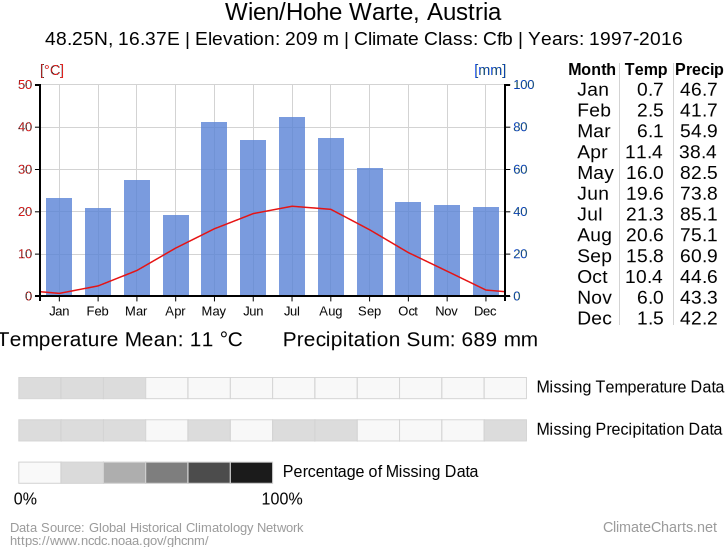
\includegraphics[width = 0.96\textwidth]{temp_maps/temp_vienna}
  	\caption{Monthly averages of temperature and precipitation data for the Hohe Warte in Vienna, Austria. (Image credit: \cite{Zepner:2020} and \emph{climatecharts.net})}
	\label{fig:temp_vienna}
\end{figure}

The photocurrent $I_{\mathrm{Ph}}$, as shown in equation \ref{eq:photo_i}, is proportional to the radiation flux $\Phi_{\mathrm{GEN}}$ -- introduced in the previous section -- with $S = \mathrm{const.}$ being the \emph{sensitivity} of the PVC.
\begin{center}
	\begin{equation} \label{eq:photo_i}
		 I_{\mathrm{Ph}} = S \, \Phi_{\mathrm{GEN}} 
	\end{equation}
\end{center}
If now is accepted, that the diode's reverse current $I_{\mathrm{S}}$ is small compared to the photocurrent $I_{\mathrm{Ph}}$ ($I_{\mathrm{S}} \ll I_{\mathrm{Ph}}$), so that $I_{\mathrm{S}} + I_{\mathrm{Ph}} \approx I_{\mathrm{Ph}}$ applies, the relationship $I_{\mathrm{SC}} \approx I_{\mathrm{Ph}}$ can be derived. $I_{\mathrm{SC}}\left(\vartheta\right)$ from equation \ref{eq:i_short_circuit} can then be approximated to:
\begin{center}
	\begin{equation} \label{eq:i_short_circuit_phi_gen}
		I_{\mathrm{SC}}\left(\vartheta,\Phi\right) \approx \underbrace{S \, \Phi_{\mathrm{GEN}}}_{I_\mathrm{Ph}} \, \left[ 1 + \mathrm{TC}\left(I_{\mathrm{SC}}\right) \cdot \left(\vartheta_{\mathrm{PVC}} - \vartheta_{\mathrm{STC}} \right) \right]
	\end{equation}
\end{center}
And since $S$ is a constant value it can be calculated, using the relationship $\Phi_{\mathrm{STC}} = A_{\mathrm{PVG}} \, E_{\mathrm{STC}}$ (compare to equation \ref{eq:radiation_flux}) and the short-circuit current $I_{\mathrm{SC,STC}}$ from the PVG'S data sheet, to \cite{Mertens:2015}:
\begin{center}
	\begin{equation} \label{eq:sensitivity}
		S = \frac{I_{\mathrm{SC,STC}}}{\Phi_{\mathrm{STC}}}
	\end{equation}
\end{center}

The slope of the current-voltage characteristic from figure \ref{fig:tikz/tikz_PVG_curve} is presented in equation \ref{eq:du_pvg}.
\begin{center}
	\begin{equation} \label{eq:du_pvg}
		 \frac{\mathrm{d} U_{\mathrm{PVG}}}{\mathrm{d} I_{\mathrm{PVG}}} = - N_{\mathrm{PVC}} \left( \frac{U_{\mathrm{T}}}{I_{\mathrm{Ph}} - I_{\mathrm{PVG}} + I_{\mathrm{S}}}+ R_{\mathrm{PV}} \right)
	\end{equation}
\end{center}
Based on this equation, for $I_{\mathrm{PVG}} = 0\mathrm{A}$ and $I_{\mathrm{S}} \ll I_{\mathrm{Ph}}$, the thermal voltage $U_{\mathrm{T}}$ can be approximated to:
\begin{center}
	\begin{equation} \label{eq:u_thermal}
		 U_{\mathrm{T}} \approx - I_{\mathrm{SC}}\left(\vartheta,\Phi\right) \, \frac{M + N_{\mathrm{PVC}} \, R_{\mathrm{PV}}}{N_{\mathrm{PVC}}} \text{, }
	\end{equation}
\end{center}
with the slope of the current-voltage characteristic for $I_{\mathrm{PVG}} = 0\mathrm{A}$:
\begin{center}
	\begin{equation} \label{eq:du_pvg_M}
		 M = \frac{\mathrm{d} U_{\mathrm{PVG}}}{\mathrm{d} I_{\mathrm{PVG}}} \left( I_{\mathrm{PVG}} = 0\mathrm{A} \right) \text{.}
	\end{equation}
\end{center}

The electrical power $P_\mathrm{PVG}$ of the PVG can be calculated by multiplying eqaution \ref{eq:u_of_i} by $I_\mathrm{PVG}$. This results in:
\begin{center}
	\begin{equation} \label{eq:p_pvg}
		 P_{\mathrm{PVG}}\left(I_{\mathrm{PVG}}\right) = I_{\mathrm{PVG}} \, N_{\mathrm{PVC}} \left( U_{\mathrm{T}} \, \ln \left( \frac{I_{\mathrm{Ph}} - I_{\mathrm{PVG}} + I_{\mathrm{S}}}{I_{\mathrm{S}}} \right) - I_{\mathrm{PVG}} \, R_{\mathrm{PV}} \right) \text{.}
	\end{equation}
\end{center}
And its derivative with respect to $I_{\mathrm{PVG}}$ is:
\begin{center}
	\begin{equation} \label{eq:dp_pvg}
		\begin{aligned}
			&\frac{\mathrm{d} P_{\mathrm{PVG}}}{\mathrm{d} I_{\mathrm{PVG}}} = \\
			& = N_{\mathrm{PVC}} \left[ U_{\mathrm{T}} \, \ln \left( \frac{I_{\mathrm{Ph}} - I_{\mathrm{PVG}} + I_{\mathrm{S}}}{I_{\mathrm{S}}} \right) - I_{\mathrm{PVG}} \left( \frac{U_{\mathrm{T}}}{I_{\mathrm{Ph}} - I_{\mathrm{PVG}} + I_{\mathrm{S}}} + 2 R_{\mathrm{PV}} \right) \right] \text{.}
		 \end{aligned}
	\end{equation}
\end{center}
With equation \ref{eq:u_of_i} for $I_\mathrm{MPP}$, and becuase equation \ref{eq:dp_pvg} is $0\mathrm{V}$ for $P_\mathrm{MPP}$, it can furthermore be written:
\begin{center}
	\begin{equation} \label{eq:u_mpp_with_dp_zero}
		\begin{gathered}
		 U_{\mathrm{PVG}}\left(I_{\mathrm{PVG}} = I_{\mathrm{MPP}}\right) - \underbrace{\frac{\mathrm{d} P_{\mathrm{PVG}}}{\mathrm{d} I_{\mathrm{PVG}}} \left( I_{\mathrm{PVG}} = I_{\mathrm{MPP}} \right)}_{0\mathrm{V}} = U_{\mathrm{MPP}} \\ = I_\mathrm{MPP} \, N_\mathrm{PVC} \left( \frac{U_\mathrm{T}}{I_\mathrm{Ph} - I_\mathrm{MPP} + I_\mathrm{S}} + R_\mathrm{PV} \right) \text{.}
		 \end{gathered}
	\end{equation}
\end{center}
Inserting equation \ref{eq:u_thermal} into equation \ref{eq:u_mpp_with_dp_zero} and assuming that $I_{\mathrm{S}} \ll I_{\mathrm{Ph}}$, then $R_\mathrm{PV}$ can be approximated to:
\begin{center}
	\begin{equation} \label{eq:r_pv}
		  R_\mathrm{PV} \approx \frac{I_\mathrm{MPP} \left( I_{\mathrm{SC}}\left(\vartheta,\Phi\right) - I_\mathrm{MPP}\right) + M \, I_\mathrm{MPP} \, I_{\mathrm{SC}}\left(\vartheta,\Phi\right)}{I_\mathrm{MPP} \, N_\mathrm{PVC} \left( I_{\mathrm{SC}}\left(\vartheta,\Phi\right) - I_\mathrm{MPP}\right) - I_\mathrm{MPP} \, I_{\mathrm{SC}}\left(\vartheta,\Phi\right) }
	\end{equation}
\end{center}

The diode's reverse current $I_\mathrm{S}$ can be approximated by using equation \ref{eq:i_of_u} for $U_\mathrm{PVG} = U_\mathrm{OC}\left(\vartheta,\Phi\right)$ with $I_{\mathrm{S}} \ll I_{\mathrm{Ph}}$, as shown in equation \ref{eq:i_s_reverse_current}.
\begin{center}
	\begin{equation} \label{eq:i_s_reverse_current}
		 I_\mathrm{S} \approx I_{\mathrm{SC}}\left(\vartheta,\Phi\right) \, \exp \left( - \frac{U_{\mathrm{OC}}\left(\vartheta,\Phi\right)}{N_\mathrm{PVC} \, U_\mathrm{T}} \right)
	\end{equation}
\end{center}

%% END ARCHIVE 2